\section{Experimental Setup}
\label{sec:brewrc-setup}

\begin{figure}[t!]
	\vspace{-10px}
	\centering
	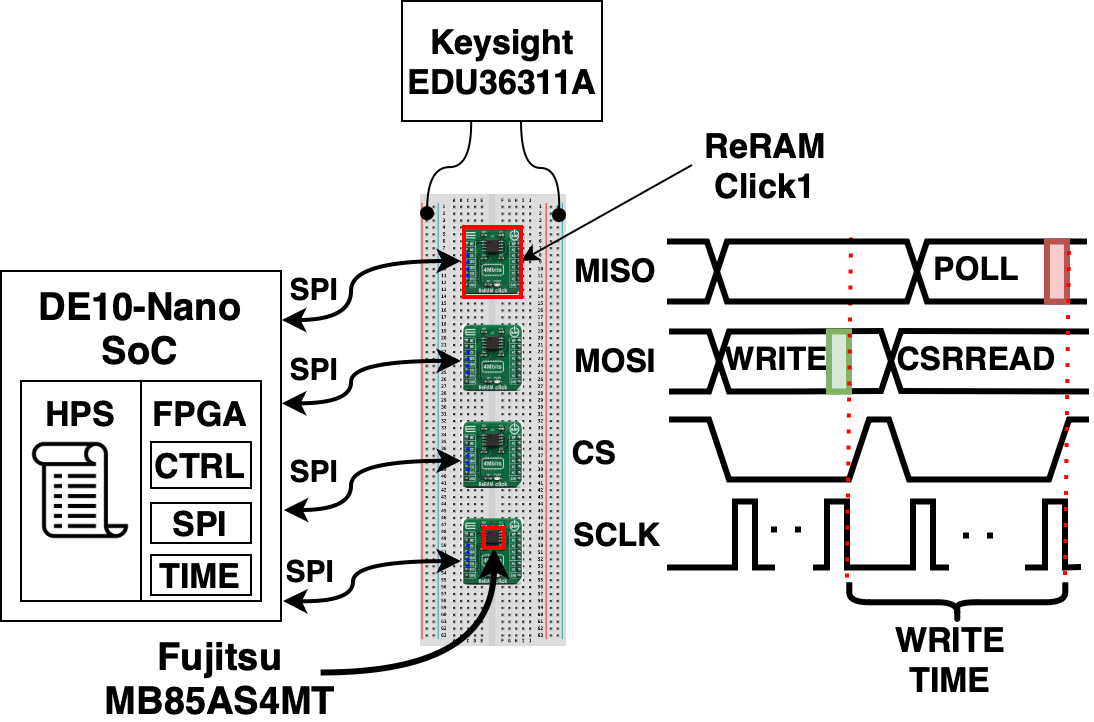
\includegraphics[width=0.75\linewidth]{img/experimental_setup.png}
	\caption{ReRAM memory instrumentation and WRITE transaction timing. An Altera DE10-Nano SoC FPGA system communicates to several Fujitsu MB85AS4MT (or MB85AS8MT) ReRAM memories via SPI. The ReRAM modules are connected to a separate EDU36311A DC power supply. The DE10-Nano is configured to measure the duration of SPI WRITE transactions \label{fig:expt-setup}.}
\end{figure}

The experiments in this chapter are performed on four samples each of
two ReRAM products from RAMXeed (formerly Fujitsu Semiconductor Memory
Solutions Ltd.). Device specifications are listed in
Table~\ref{tab:reram_spec}.

\begin{table}[t!]
	\centering
	\caption{RAMXeed ReRAM device comparison.}
	\label{tab:reram_spec}
	\renewcommand{\arraystretch}{1.0}
	\setlength{\tabcolsep}{3.5pt}
	\begin{minipage}{0.98\columnwidth}
		\centering
		\begin{tabular}{lcccc}
			\toprule
			\textbf{Device}    & \textbf{Capacity}  & \textbf{SPI} $\mathbf{f_{\max}}$ &
			\textbf{Endurance} & \textbf{Buf. Size}                                                              \\
			\midrule
			\textbf{MB85AS4MT} & 4\,Mb              & 5\,MHz                           & 1.2M\,Times/B  & 256\,B \\
			\textbf{MB85AS8MT} & 8\,Mb              & 10\,MHz                          & 1M\,Times/4\,B & 256\,B \\
			\bottomrule
		\end{tabular}
	\end{minipage}
	% \vspace{-.5cm}
\end{table}


Each experiment collects write latencies $t_w$ corresponding to a set of
applied test vectors. Each write is committed to the device over a SPI
interface by de-asserting chip-select following the last byte of a
\texttt{WRITE} operation. $t_w$ is measured from the time the write
transaction is committed to the time the write-in-progress (WIP) bit of
the STATUS register is cleared. Measurements of $t_w$ are quantized by
the minimum time required to check for write completion ($\Delta t$),
which is defined as the time between successive read status register
(RDSR) operations:
\begin{equation}
	\Delta t = \frac{8}{f_{SPI}}.
\end{equation}
The RDSR can be polled continuously by holding chip-select while driving the SPI clock; the status register is returned every 8 SPI clock cycles. SPI interfaces are operated at the maximum frequency defined in the device specification. The minimum $\Delta t$ of the MB85AS4MT and MB85AS8MT memories are therefore $1.6\,\mu$s and $0.8\,\mu$s, respectively.
SPI transactions are applied and timed using a Terasic DE10-Nano Cyclone V SoC FPGA development kit. For each write operation, a hardware counter on the FPGA captures $t_w$ and pushes it to a response FIFO. The FPGA is used primarily to scale experiments across multiple device samples in parallel. Prior works have demonstrated equivalent timing capabilities using microcontrollers~\cite{tolga2024trng, ferdaus2024hiding}.
